\section{Range of forces}
\subsection{Massless field}
Start from the relativistic form of the Schr\"odinger equation: Klein-Gordon equation
\begin{equation*}
(\frac{1}{c^2}\frac{\partial^{2}}{\partial t^2}-\vec{\nabla}^2)\psi+\frac{m^2c^2}{\hbar^2}\phi=0
\end{equation*}
Here $\phi$, just like $\psi$ in previous sections, represents a wave-function. Turns out we can think of $\phi$ also related to a field. Why? Well consider the simple case of a time-independent massless and spherically symmetric $\phi$ for simplicity. We then have
\[m=0,\frac{\partial\phi}{\partial t}=0,\nabla^2\phi\rightarrow \frac{1}{r}\frac{d^2}{dr^2}(r\phi)
\]
so the Klein-Gordon equation becomes
\[
\frac{d^2}{dr^2}(r\phi)=0
\]
yielding $\phi\propto\frac{1}{r}$. In fact $\nabla^2\phi=0$ IS Maxwell's equation for an Electric potential in the vacuum! So $\phi$ really is your standard Electric potential ie
\[\phi=\frac{Q}{4\pi\epsilon_{0}r}\] and consequently $\nabla\phi$ your electric field! The coupling strength can be identified as $\frac{Q}{4\pi\epsilon_{0}}$.

\paragraph{What does all this tell us?}We can think of $\phi$ as being the potential of the force mediated by a massless particle (e.g the photon\footnote{This is not quite correct, the Klein-Gordon equation describes particles with no intrinsic angular momentum so it cannot completely describe the photon which does carry angular momentum.}). The influence of this potential goes as $\frac{1}{r}$, therefore the range of this field is infinite as $\phi\to0$ for $r\to\infty$. 

\subsection{Massive field}
\label{sec:massive_field}
Just as for the massless case we can start from the Klein-Gordon equation where for simplicity we assume $\phi$ is a time-independent and spherically symmetric but now $\phi$ does have a mass. Therefore the Klein-Gordon equation becomes
\[
\frac{d^2}{dr^2}(r\phi)=\frac{m^2c^2}{\hbar^2}(r\phi)
\]
The solution to this equation is
\[
\phi=g\frac{e^{-rmc/\hbar}}{r}
\]
where $g$ represents and coupling strength. This for of $\phi$ is known as the ``Yukawa-potential''. It can be thought as the potential of a force mediated by a massive particle. There is an interesting effect here:
\begin{enumerate}
\item If $\frac{mc}{\hbar}$ is small then $\frac{1}{r}$ dominates $\to$ Long range
\item If $\frac{mc}{\hbar}$ is large then the exponential dominates $\to$ Short range
\end{enumerate}
A good example of this is the weak-interaction. Last year you learnt that the weak-interaction is mediated by massive gauge bosons, the $W$ and $Z$ with masses of 80 and 91~GeV respectively. %Consider the decay of the pion 
%\begin{center}
%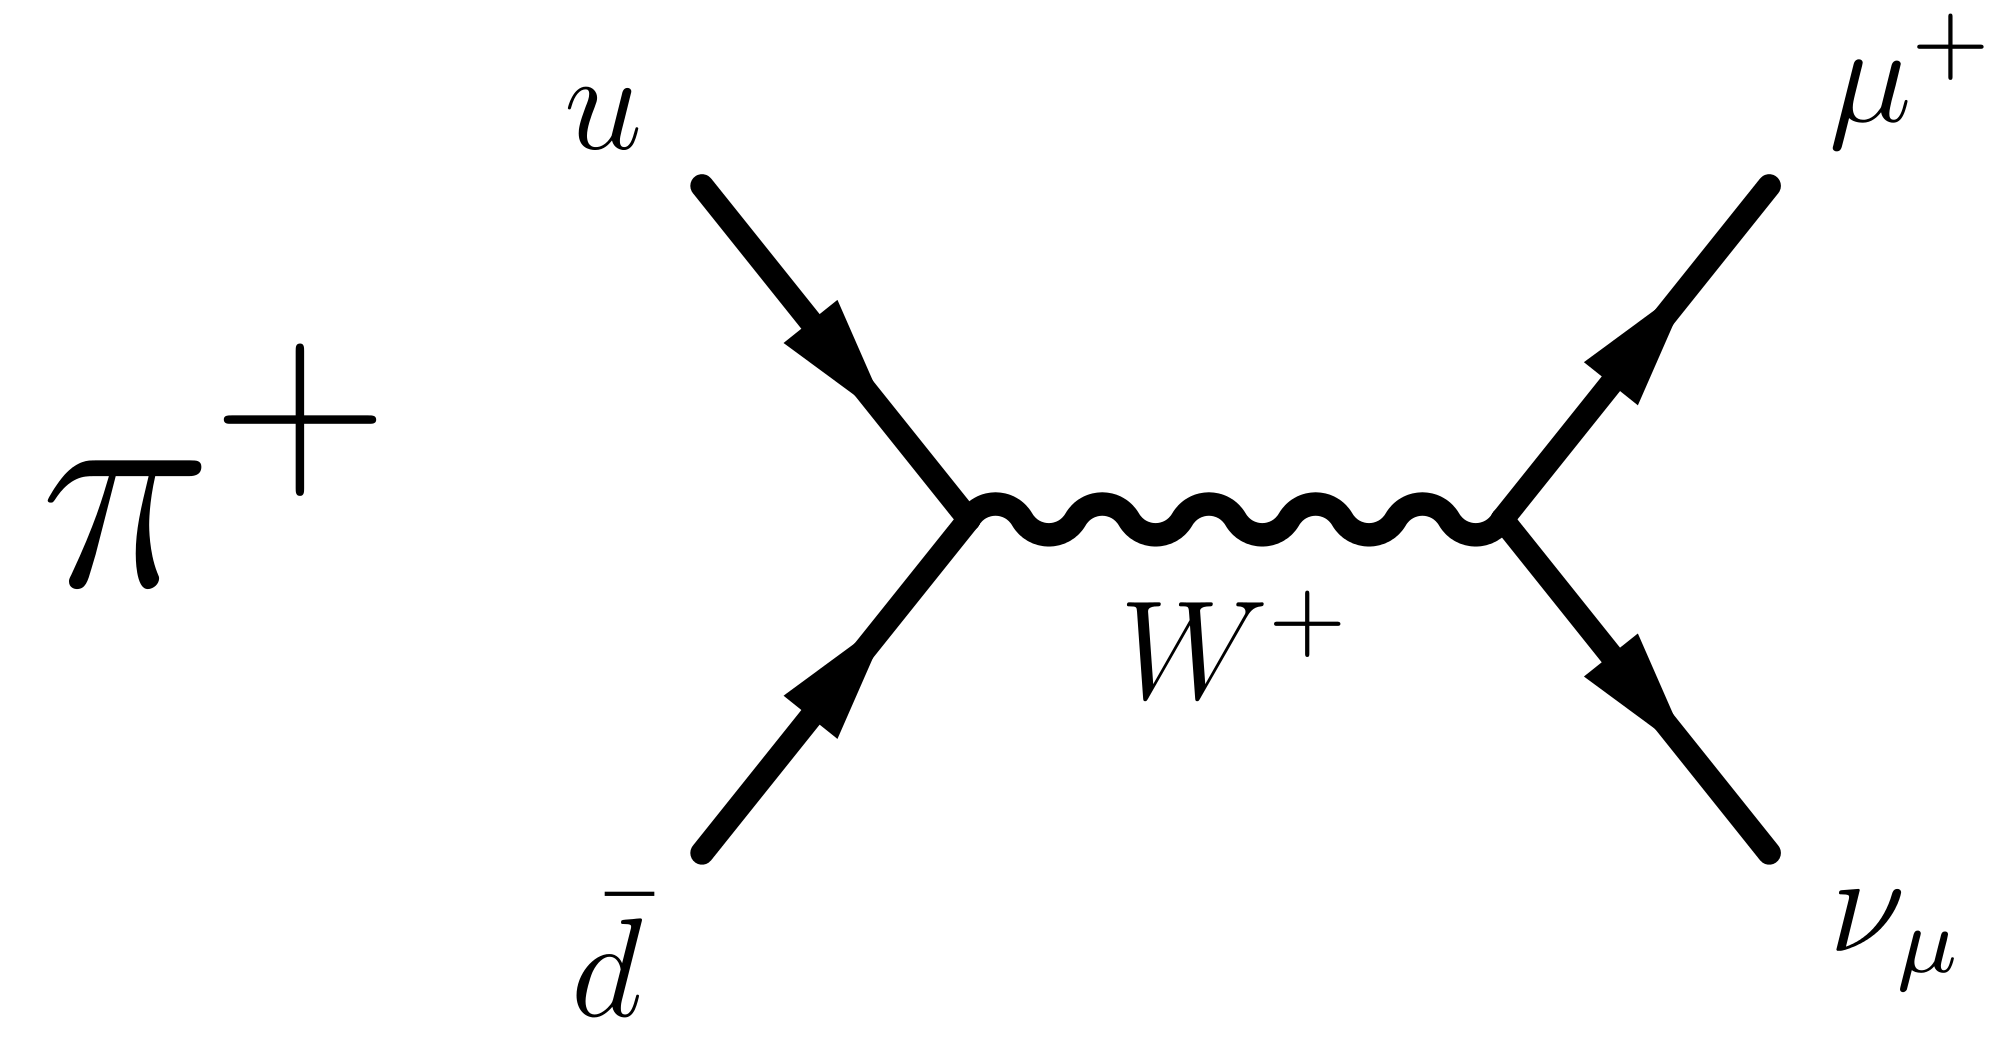
\includegraphics[width=0.5\textwidth]{fig/forcerange/weak_feyn_example.png}
%\end{center}
So the Weak coupling strength is larger than the EM coupling however the shorter range of the Weak force means that the Weak force appears weaker than the EM force. The Yukawa-potential is another way of understanding the coupling strength of the weak interaction\footnote{This approach leads to the explanation of the coupling strength of the Weak interaction due to the presence of a propagator, that you were taught last year (Sec~3.3 of \texttt{PHYS22040} course notes).}.

\subsection{Summary of fundamental forces and their strengths}
\begin{center}
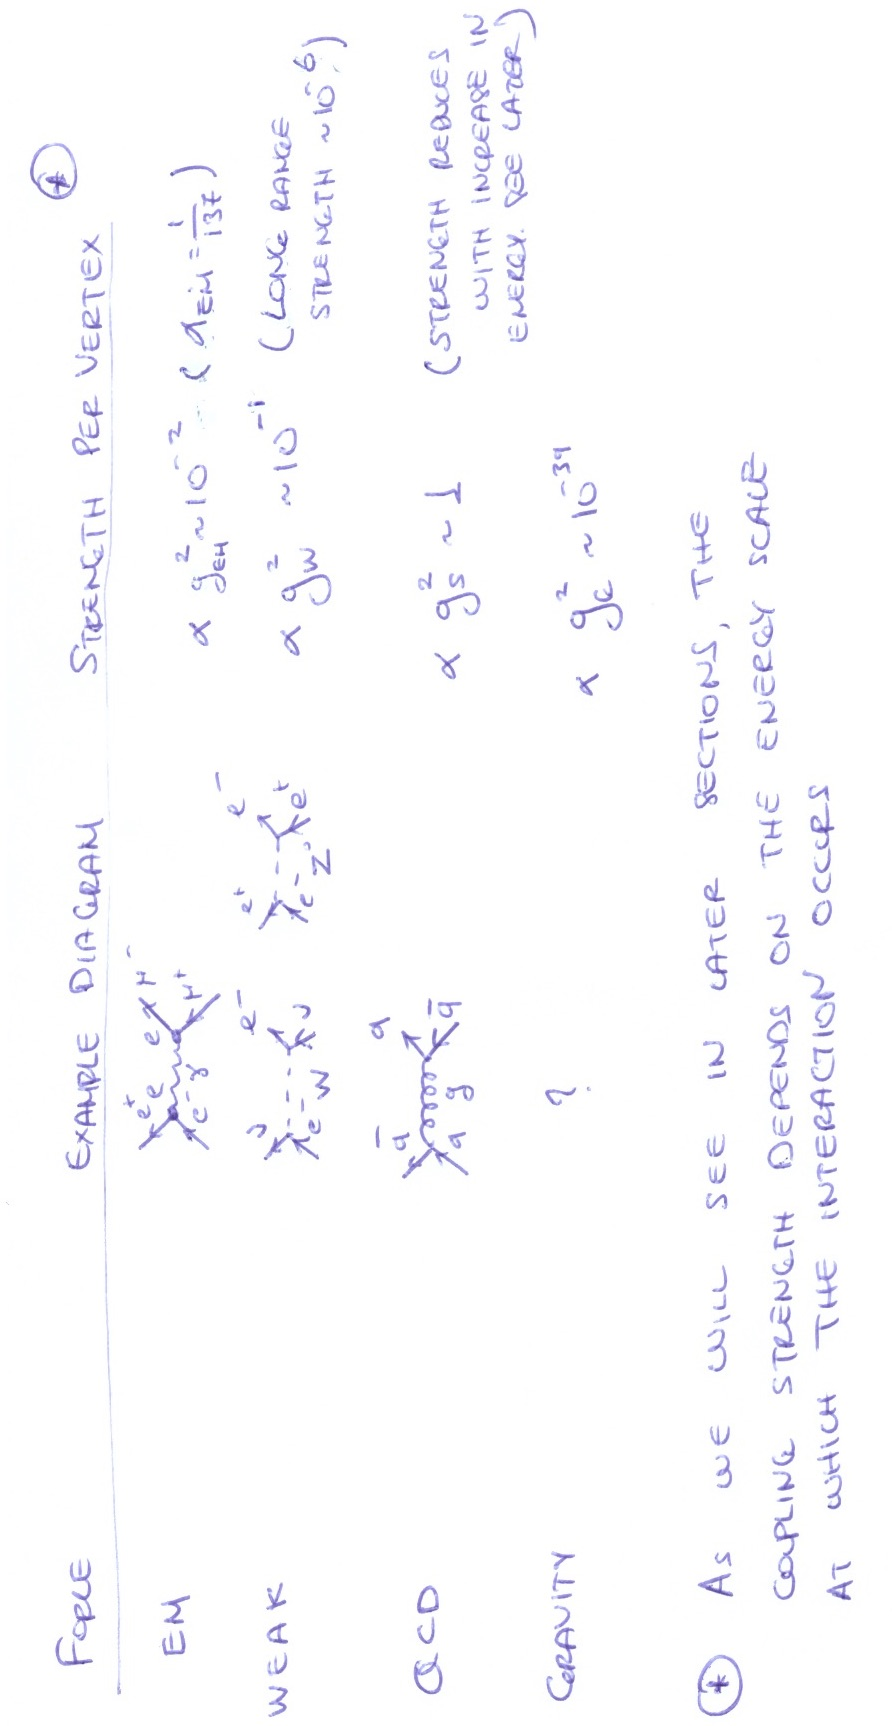
\includegraphics[angle=270,width=0.99\textwidth]{fig/forcerange/forces.jpg}
\end{center}
The various $g_i$ correspond to the coupling associated to each vertex. The probability for a particular vertex to occur is proportional to $g_{i}^2$. The $g_i$ coupling is in turn proportional to the charge of each particle under the force in question. For example the EM charge of the electron and the muon is $e$. 

